\documentclass{article}

% Language setting
% Replace `english' with e.g. `spanish' to change the document language
\usepackage[english]{babel}

% Set page size and margins
% Replace `letterpaper' with `a4paper' for UK/EU standard size
\usepackage[letterpaper,top=2cm,bottom=2cm,left=3cm,right=3cm,marginparwidth=1.75cm]{geometry}

% Useful packages
\usepackage{amsmath}
\usepackage{graphicx}
\usepackage[colorlinks=true, allcolors=blue]{hyperref}
\usepackage{subfig}
\usepackage[figuresleft]{rotating}

\title{Porovnání výkonu MongoDB vs InfluxDB pro time-series data}
\author{Martin Skalický}

\begin{document}
\maketitle

\section{Úvod}

Ve své bakalářské práci s tématem IoT Platforma s webovým rozhraním jsem využil MongoDB jako hlavní databázi pro ukládání všech dat a to včetně dat získávaných z IoT zařízení. Jedná se o poměrně velké množství, které roste lineárně s přidáváním dalších zařízení - každé zařízení pošle přibližně 600 zpráv každý den a platforma by měla zvládnout obsloužit stovky až tisíce zařízení. Od prvopočátku jsem počítal s jistými výkonostními limity při využití MongoDB na tento typ dat a již při návrhu jsem řešil jisté optimalizace, abych tento dopad minimalizoval.

V nedávné době jsem ukládání dat z IoT zařízení přesunul na databázi InfluxDB, který by měla být pro tento typ dat mnohem vhodnější a v rámci této práce provedu analýzu nad reálným výkonostním dopadem této změny.

\section{Představení databází}

\subsection{MongoDB}

MongoDB je dokumentová databáze, která se řadí mezi takzvané NoSQL databáze. Na rozdíl od klasických relačních databází nepoužívá fixní schéma ale dynamické a dokumenty (záznamy) jsou ukládány ve formátu BSON - jedná se v podstatě o známý formát JSON ze světa jazyka JavaScript, ale v binární podobě.

Databáze velmi vyniká svojí flexibilitou díky absenci fixních schémat. Má rozsáhlý dotazovací jazyk využívající vlastní jazyk "MongoDB Query Language", který dokonce podporuje i přímé spouštění vlastních JavaScript funkcí v databázi. Pro komplexní zpracování dat umožňuje spouštění agregací. 

Od verze 5 je přidáná nativní podpora pro časové řady avšak v rámci této práce se budu zabývat starší verzí 4, která byla původně využita pro již zmíněnou IoT Platformu.

\subsection{InfluxDB}

Databáze InfluxDB byla speciálně navržena pro ukládání a zpracování časových řad. Je napsaná v jazyce GO a první verze byla vydána až v roce 2013 (MongoDB bylo vydáno v 2009). Tím, že je databáze nativné určena pro časové řady, tak data se vkládájí jako body, které nesou časové razítko, hodnoty a textové značky (tags). Značky jsou použity pro označení, že více bodů spolu souvisí. Pro dotazování jsou podporovány dva přístupy: jazyk podobný SQL (InfluxQL) nebo vlastní funkcionální jazyk Flux. 

V základu obsahuje i webové rozhraní, ve kterém lze kromě psaní dotazů i přímo data vizualizovat pomocí různorodých grafů. Toto rozhraní je velmi příjemné, ale po chvílí jsem začal narážet na limitace, protože se jedná o jednodušší zpracování co se týče možností vlastních úprav. Pro větší přispůsobení je potřeba sáhnout po lepším analytickém nástroji jako Kibana či Grafana, které přímo podporují napojení na InfluxDB.

\section{Ukládání dat}
Tato kapitola popisuje způsob uložení časových řad do obou databází včetně schémat a datových typů.

Datovou doménou ukládaných dat jsou IoT zařízení. Každé zařízení je dále hierarchicky rozděleno na věci a každá věc na vlastnosti. Příklad dělení: zařízení - auto má věci: motor a kola. Motor má vlastnosti: tlak, teplotu a stav oleje. Kola mají vlastností: tlak v prvním kole, druhém atd... Tedy zařízení odpovídá fyzickému zařízení, věci jsou logické rozdělení zařízení a vlastnosti jsou již fyzické senzory či ovládací prvky. Zda se jedná o prvek, který odesílá údaje (senzor) či ovládací prvek, který přijímá povely z platformy je z pohledu ukládání dat jedno a to samé. 

Každé zařízení, věc i vlastnost má unikátní ID v dané kategorii, které bude využit v databázi pro identifikaci. Cílem je ukládat všechna data, která zařízení odeslala s časovým razítkem. Pro potřeby Platformy získat graf průběhu za posledních 24 hodin a pro potřeby datové analýza dokázat zpracovat statistiky za libovolné časové úseky pro datové typy: \it{boolean}, \it{string}, \it{float}, \it{integer}. Pro číselné datové typy např. průměr či maximální/minimální hodnoty.


\subsection{MongoDB}
Jako tzv. \it{schemaless} databáze nevyžaduje MongoDB pevně definované schéma avšak na aplikační úrovni je potřeba nějaké schéma vytvořit, aby data byla ukládána v určitém formátu a šlo se na ně později dotazovat. Následující ukázky budou využívat knihovnu Mongoose pro definice schémat pro MongoDB na aplikační úrovni - kromě samotných schémat knihovna umí řešit převody datových typů, validace a dává k dispozici API s vyšší abstrakcí postavené nad nativním \it{MongoDB query}.

Naivní způsob uložení pro někoho kdo přijde ze světa relačních databázích by mohl být jednoduše co záznam to nový dokument, kde jeden záznam odpovídá jedné získané hodnotě, jejímž klíčem bude jedno zařízení, věc, vlastnost a časové razítko. Tedy takovéto schéma:

\begin{figure}[htbp]
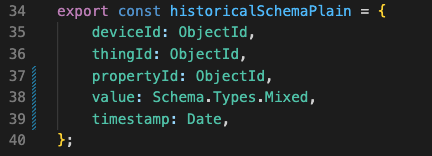
\includegraphics[width=8cm]{images/naive_schema.png}
\centering
\caption{Naivní uložení každé hodnoty jako jako dokument}
\end{figure}

Tento způsob by však dosahoval velice špatných výkonnostních výsledků. Síla MongoDB dotazovací jazyka je v možnostech dotazování na vnořené struktury v dokumentech. V tomto případě by vznikalo obrovské množství miniaturních dokumentů na což jsou stavěné relační databáze - na velké množství malých řádek ale pro MongoDB by toto nefungovalo - při získávání velkého množství dokumentů bude docházet k obrovské zážeži na disky, protože dokument je uložený jako celek avšak dokumenty jsou rozházené na různých místech a dochází k hodně IOPS, což bude především u magnetických disků problém.

Další možností je vytvořit jeden dokument pro každou vlastnost a hodnoty jednoduše přidávat do pole. Tento návrh je o trochu lepší než předchozí, ale zde bychom brzy narazily na limit maximální velikosti jednoho dokumentu, který je stanoven na 16~MB. Také ne všechny vlastnosti generují stejné množství dat a velikosti dokumentů by byly velmi nevyvážené - některé by obsahovali desítky hodnoty a jiné stovky tisíc. MongoDB v dokumentaci nedoporučuje pracovat s obrovskými poli z důvodu výkoností náročnosti při častém přidávání či odebírání prvků kvůli realokaci paměti.

\begin{figure}[htbp]
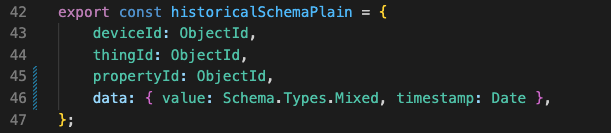
\includegraphics[width=10cm]{images/basic_schema.png}
\centering 
\caption{Uložení hodnot do pole}
\end{figure}

Pro uložení dat bude tedy potřeba určitý kompromis mezi řešeními uvedenými výše. Při návrhu jsem se inspiroval z příspěvku, které mělo MongoDB uvedeno na svém blogu pro ukládání podobného typu dat, ale bohužel se mi již nepodařilo dohledat tento zdroj. Návrch schématu se ve velké míře ohledně optimalizací odvíjel od toho, jaké dotazy se nejčastěji budou provádět. Řešení je založeno na rovnoměrné distribuci dat do dokumentů o určité maximální velikosti. Pro zápis hodnot vždy vznikne dokument, který je unikátní pro určité zařízení a věc. Tento dokument se plní hodnotami z příslušných věcí až se dosáhne určitého celkového množství hodnot, která je definována fixní hodnotou. Následně je vytvořen dokument nový pro ukládání a až je zase naplněn, tak se proces opakuje. Prahová hodnota pro počet hodnot byla odhadnuta vzhledem k předpokládanému počtu zatížení na 200 - průměrně 3 vlastnosti, každá 3 zprávy za hodinu - \(3*3*24 = 214\). Celá platforma je koncipována primárně pro náhledy na data za celý den, z toho jsem vycházel při návrhu primárního klíče, že do něho přibude i datum. Díky tomu bude snadné postavit index, který seskupí dokumenty podle data a nad tím provádět analýzy. Dokument také obsahuje časová razítka první a poslední hodnoty, které dokument obsahuje.

Dokument je strukturován tak, že pod klíčem yit{properties} se nachází objekt, ve kterém jsou klíče identifikátory jednotlivých vlastností. Důvod proč je použit objekt s klíči a ne pole, je kvůli jednoduššímu psaní dotazů a mutacím přes tečkovou notaci. Pod jednotlivými vlastnostmi se pak nachází klíč \it{samples}, který obsahuje samotná data s časovým razítkem a \it{nsamples} obsahuje počet dat. Protože uživatelské rozhraní má často zobrazovat základní statistiky jako minimun, maximum a průměr, tak aby se tyto hodnoty nemuseli počítat s každým dotazem přes všechna data, tak jsou průběžně počítány - tomu odpovídají políčka: \it{min}, \it{max}, \it{sum}. Součet je ještě navíc dělen na noc a den, aby bylo možné počítat denní, noční a celkový průměr (přelom noc a den je definován fixní hodnotou na aplikační úrovni).


\begin{figure}[htbp]
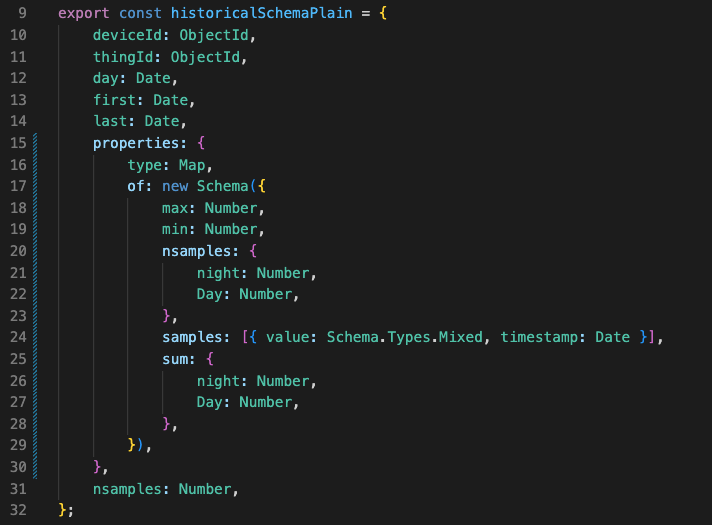
\includegraphics[width=10cm]{images/full_schema.png}
\centering 
\caption{Výsledné schéma}
\end{figure}



\subsection{InfluxDB}
Tato databáze je speciálně navržena pro časové řady a proto také způsob ukládání hodnot je mnohem přímočařejší. Nativní záznam pro InfluxDB je tzv. "bod", který označuje hodnotu v čase. Pro identifikaci bude opět mít identifikátory zařízení, věci a vlastnosti. Navíc oproti MongoDB bude mít ještě název zařízení - toto není nutné kvůli dotazování, ale kvůli pozdější tvorbě grafů, aby se dalo lépe pracovat se záznamy a na první pohled bylo možné rozpoznat jakému zařízení data patří. Protože InfluxDB má tzv. "query builder", který umožňuje základní tvorbu dotazů jednoduchým "naklikáním" a takto to bude lépe viditelné i bez znalosti dlouhého identifikátoru zařízení.

\begin{figure}[htbp]
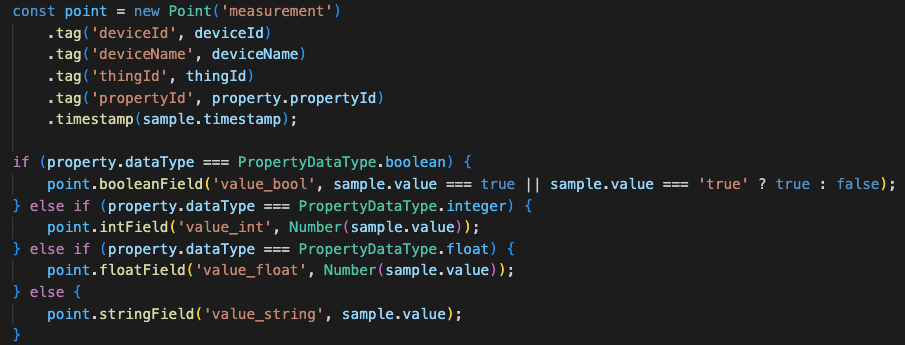
\includegraphics[width=15cm]{images/influx_point.png}
\centering 
\caption{Uložení jedné hodnoty} 
\end{figure}

Na ukázce je viditelné vytváření záznamu s oficiálním SDK pro NodeJS. Vytvoří se bod, kterému nastavuji tagy, které odpovídají jednotlivým identifikátorům - pomocí tagů je pak možno jednoduše filtrovat. Vždy je potřeba přidat časové razítko a následně nastavit hodnotu. Tím, že Platforma podporuje více datových typů a InfluxDB vynucuje pro určitý klíč s hodnotou vždy stejný datový typ, tak jsem musel pro různé datové typy použít různé hodnoty klíče: \it{value\_bool}, \it{value\_int}, \it{value\_float}, \it{value\_string}.

\section{Experimentální část}
Testování bude provedeno na virtualizovaném Ubuntu Desktop 20.04 LTS pomocí Gnome Boxes na hostitelském systému Fedora Workstation 36 - přidělena 2 CPU (Ryzen 3600), ram 2 GB, disk Sata SSD. Nainstalované databáze: InfluxDB v2.5.1 , MongoDB v4.4.18. Všechny naměřené hodnoty uvedené v této práci jsou průměrem z pěti opakování. Pokud nebude uvedeno jinak, tak dotazy jsou spuštěny nad MongoDB bez přidaných indexů avšak InfluxDB si vytváří automaticky index nad časem a značkami bodů (time and tags).

Data nad kterými budou prováděny dotazy jsou získaná z běžící instance IoT Platformy, kterou používám pro osobní účely - jsou na ni připojená zařízení: elektrická brána, lust, 2x led pásek, vnitřní teploměr, venkovní meteostanice, 2x měřič elektrické spotřeby, Android televize, audio reciever, výřivka a enomometr. 

Data jsou získaná za období od 9. 27. 2021 do 9. 12. 2022. Do obou databází jsou nahrány stejná v příslušném formátu, který byl diskutovat v předchozí kapitole. MongoDB obsahuje 36~000 dokumentů s uloženými daty (300~MB) a InfluxDB 5~594~177 bodů. Ukázky v této kapitole budou pro MongoDB v jazyce JavaScript s knihovnou Mongoose a pro InfluxDB z nativního webového "skript editoru" s dotazy v jazyce Flux (+ ukázky grafů, které lze velmi jednoduše vytvářet v daném rozhraní).

\subsection{Dotazy}
V této sekci se podíváme na základní dotazy nad číselnými typy pro zařízení meteostanice za určitý časový úsek.

\subsubsection{Získání dat z časového intervalu}
Nejprve se podíváme na query v MongoDB. Protože jsou data ukládány do více dokumentů, tak jsou dvě možnosti jak data získat. První je využít základní query pro nalezení dokumentů a případně filtrovat pole s daty a následně na aplikační vrstvě data spojit do jedné časové řady (myšleno seřazené pole hodnot). Druhá možnost jak získat časovou řadu již přímo z databáze, tak je využít agregace, která umožní popis manipulace dat na straně DB, pomocí kterých si data spojíme do jedné časové řady.

\begin{figure}[htbp]
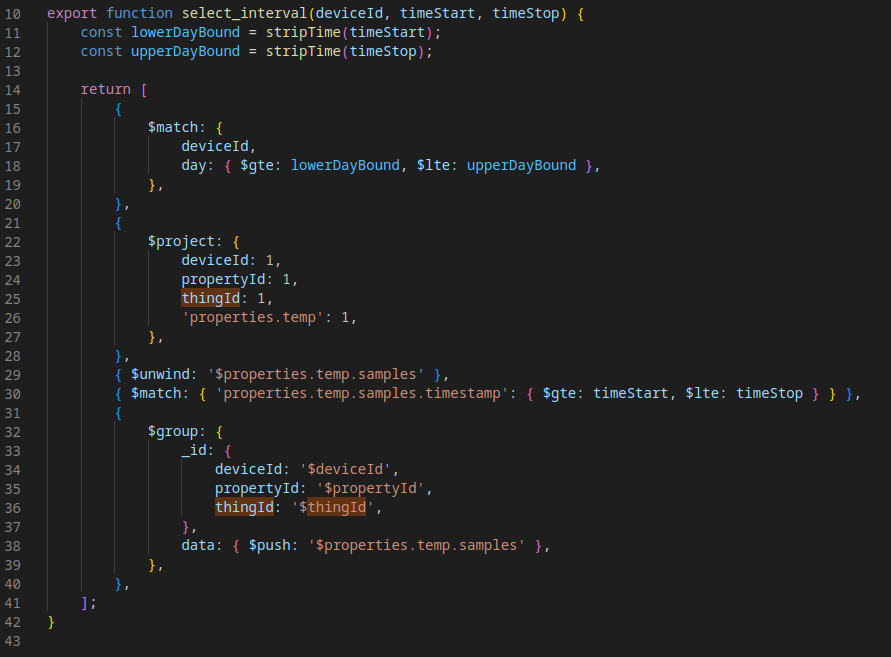
\includegraphics[width=14cm]{images/select_interval.png}
\centering 
\caption{Výběr naměřené teploty zařízení v intervalu - MongoDB \label{fig:simple:query}} 
\end{figure} 

\begin{figure}[htbp]
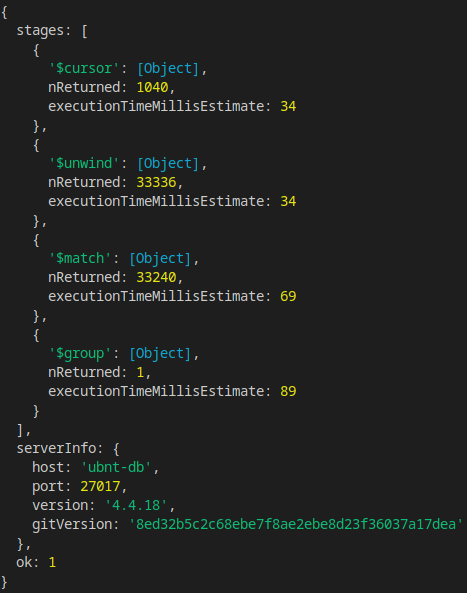
\includegraphics[width=7cm]{images/select_interval_explain.png}
\centering 
\caption{Analýza jednotlivých částí agregace - MongoDB \label{fig:simple:query:explain}} 
\end{figure} 


Agregace na ukázce \ref{fig:simple:query} definuje jednotlivé fáze výpočtu. Nejprve pomocí \it{\$match} jsou vybrány pouze dokumenty, které obsahují data pro příslušné zařízení, která byla naměřená v rozmezí dnů pro který je platný časový interval - toto filtrování se může zdát jako zbytečné protože je hodně hrubé ale přináší podstatné zvýšení výkonu. Například dotaz na data za jeden den s využitím toho hrubého filtrování trval 35~ms a bez použití toho filtrování celých 71~ms, tedy 2krát delší dobu. V další fázi agregace jsou data ořezána pro získání pouze identifikátorů a samotných hodnot s teplotou. Výsledkem těchto fází jsou dokumenty, kde každý dokument obsahuje maximálně 200 hodnot. Tyto data jsou ale omezena pro jednotlivé dny, ještě je potřeba jemněji filtrovat na úrovni času. Proto je nejprve použit \it{\$unwind}, který rozpadne pole tak, že zduplikuje dokumenty a na místo pole vloží vždy příslušný prvek z pole. Následně je možno filtrovat znovu pomocí \it{\$match} ale nyní jemněni dle času. Poslední fáze vezme všechny hodnoty a vytvoří z nich jednu výslednou časovou řadu, která již obsahuje pouze hodnoty filtrované dle časového intervalu.

Nyní se můžeme podívat podívat podrobněji na výslednou agregaci pomocí funkce \it{explain} viz. obrázek \ref{fig:simple:query:explain}. Zde je vidět časový odhad na jednotlivé kroky a počet dokumentů, které budou v dané fázi zpracovány. Nejvíce času zabere procházení všech prvků a porovnání, zda patří do výsledného intervalu či nikoliv. Index by pomohl snížit první hrubou fázi filtrování, ale v tomto kroku bohužel ne.

Následuje ukázka \ref{influx:simple:query:explain} stejného dotazu pro InfluxDB. Dotaz je mnohem jednodušší, protože InfluxDB používá plochou strukturu - každý bod je jedna hodnota s časovým razítkem. Nejprve pomocí funkce \it{range} jsou odfiltrovány hodnoty ze zadaného časového intervalu. Následují funkce pro filtraci - dle zařízení, výběr teploty a datového typu.

\begin{figure}[htbp]
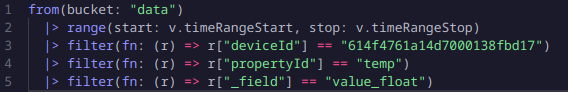
\includegraphics[width=10cm]{images/simple_query_24_infl.png}
\centering 
\caption{Výběr naměřené teploty zařízení v intervalu - InfluxDB \label{influx:simple:query:explain}} 
\end{figure} 

\begin{figure}[htbp]
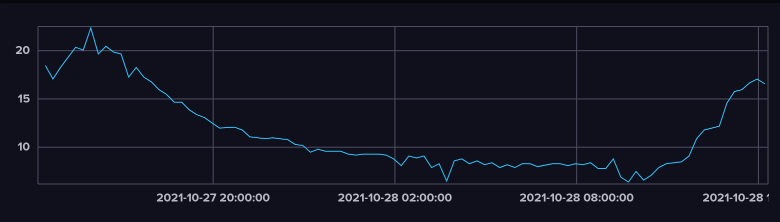
\includegraphics[width=10cm]{images/simple_query_24h.png} 
\centering 
\caption{Vizualizované hodnoty za 24h - InfluxDB} 
\end{figure}


\begin{figure}[htbp]
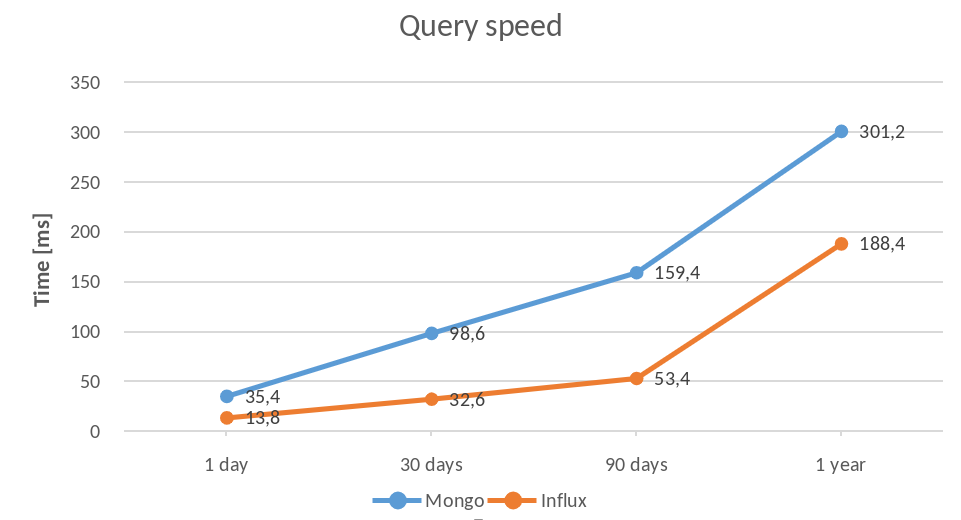
\includegraphics[width=15cm]{images/select_interval_graph.png}
\centering 
\caption{Naměřené doby zpracování dotazů pro získání dat z časového intervalu\label{graf:simple:query}} 
\end{figure}

Z grafu \ref{graf:simple:query} je viditelné, že databáze InfluxDB je přibližně o 50~\% rychlejší. Což je ovšem minimální rozdíl vzhledem k tomu, že InfluxDB by mělo být optimalizované pro časové řady na rozdíl od MongoDB a tak bych zde očekával mnohem markantnější rozdíl - především by se časová složitost neměla tak dramaticky zvyšovat s množstvím dat. Při pohledu na množství, tak za 90 dnů se získalo 8,5~k (tisíc) hodnot a za 1 rok 33~k. A právě v množství dat, která se vracejí z DB bude úzké hrdlo. Pro reálné využití pro zobrazení v grafu jsou desítky tisíc hodnot nesmyslné množství. Při pohledu na dlouhodobý průběh nás zajímá spíše trend a průběh grafu, než přesné hodnoty za každých 15 minut. Nemluvě o náročnosti vykreslení samotného grafu s tímto množství dat. A právě proto InfluxDB nativně podporuje okénkovou agregaci (window aggregation) - data jsou rozděleny dle fixní velikosti okénka a na jednotlivá okénka je aplikována agregační funkce. Výsledkem každého okénka je potom jedna hodnota, které společně tvoří výslednou posloupnost. Je to tedy způsob jak vzít velké množství dat, rozdělit je na malé skupiny, ze skupin spočítat průměr, min či max a z těchto výsledků sestavit cílovou řadu (poznámka: Mongo již okénka také podporuje od verze 5 s příchodem operátoru \it{\$setWindowFields}).


Zápis pomocí jazyka Flux je velmi jednoduchý - stačí přidat jeden řádek (viz. obrázek \ref{graf:simple:query:window}), který definuje velikost okénka a agregační funkci. Získání hodnot při velikosti okénka 1h a agregační funkcí průměr se rychlost získání odpovědi snížila o 2/3 z průměrných 188~ms na 54~ms, nyní DB vrací 1/3 hodnot z původních 33~k "pouhých" 8~k. Při nastavování velikosti okénka záleží na způsobu následného využití dat. V případě zobrazení na UI by bylo možné ještě snížit okénko až na 1 den, aby výsledkem bylo 350 hodnot (průměrná rychlost je potom 30~ms) avšak v případě strojového zpracování může být nutné získat úplně všechna neupravená data.
\begin{figure}[htbp]
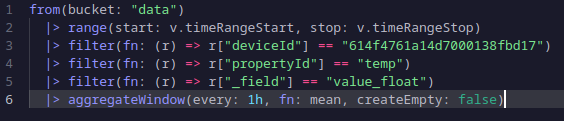
\includegraphics[width=10cm]{images/simple_query_window.png}
\centering 
\caption{Výběr naměřené teploty zařízení v intervalu s okénkem - InfluxDB\label{graf:simple:query:window}} 
\end{figure}



\subsubsection{Získání průměru hodnot dnů z časového intervalu}
V této sekci budeme porovnávat výkon pro získání průměrné hodnoty za jednotlivé dny z časového intervalu. U MongoDB porovnáme dvě řešení: naivní a využívající optimalizaci, který by znatelně měla zvýšit výkon. Zmíněná optimalizace se týká vytváření okénka na úrovni schématu. Specificky atributy \it{properties.{id}.sum,min,max,nsamples}, která jsou počítána již při ukládání hodnot do DB a jsou to tak hodnoty předpočítané  téměř na úrovni jednotlivých dnů (uměle si zde vyrábím něco jako okénko). Díky tomuto dotazy na základní statistiky pro průměr, min, max atd. se budou počítat z těchto již částečně předpočítaných atributů a sníží se tak potřebný výpočetní výkon a především I/O operace. Daní je však zde to, že je nutné pro tyto případy psát jiné dotazy, musí se s tím počítat již při návrhu schématu (nebo případně zpětně dopočítat) a zdaleka ne všechny výpočty lze takto urychlit.

První variantou je naivní řešení pro MongoDB. Jedná se o předchozí dotaz viz. \ref{fig:simple:query} s drobnou změnou, kde místo operátoru \it{\$push} je využit operátor pro výpočt průměru \it{\$avg} a do identifikátoru pro seskupení měření \it{\$group} je přidán ještě atribut \it{day}, aby se průměr počítal pro každý den zvlášť.

Nyní se podívejme na optimalizovanou MongoDB variantu viz. obrázek \ref{mongo:basic:avg}. První \it{\$match} fáze je stejná jako předchozí, v projekci nyní nejsou vybrány data, ale pouze napočítané součty a počty hodnoty. Identifikátor seskupení opět obsahuje den a pro každou skupinou jsou vypočteny celkové součty průměru a počtu hodnot za den a noc. Z výstupu této fáze je vypočten celkový průměr podělením celkového součtu ku počtu hodnot.


\begin{figure}[htbp]
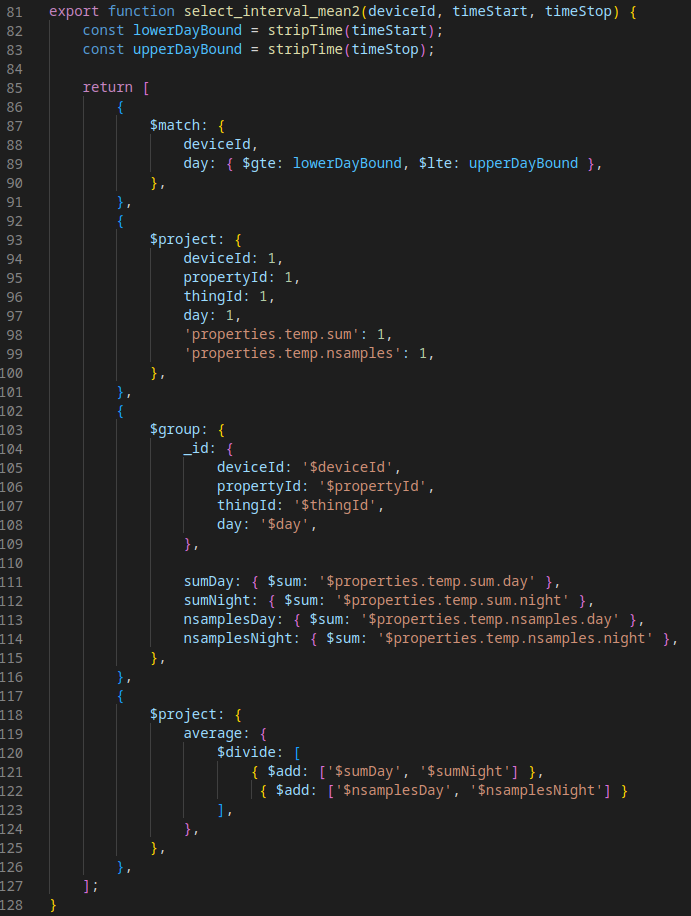
\includegraphics[width=10cm]{images/mongo_basic_avg.png}
\centering   
\caption{Výběr denních průměrů teploty zařízení v intervalu - MongoDB \label{mongo:basic:avg}} 
\end{figure}


\begin{figure}[htbp]
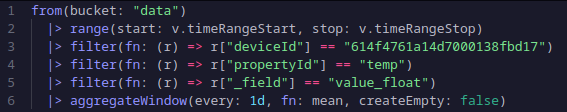
\includegraphics[width=10cm]{images/influx_simple_avg.png}
\centering   
\caption{Výběr denních průměrů teploty zařízení v intervalu - InfluxDB \label{influx:basic:avg}} 
\end{figure}

Řešení v InfluxDB je mnohem jednodušší. K dotazu s filtrací stačí přidat výběr okénka, které se nastaví na velikost 1 den a nastaví se agregační funkce pro průměr (\it{mean}) viz. ukázka \ref{influx:basic:avg}.


\begin{sidewaysfigure}

    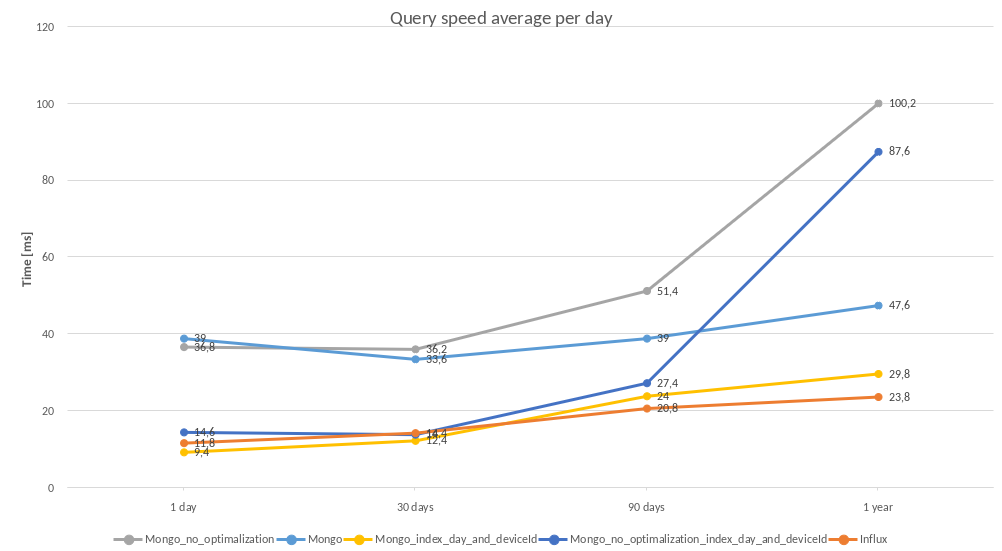
\includegraphics[width=20cm]{images/query_avg_all_graph.png}
    \centering   
    \caption{Naměřené doby zpracování dotazů pro získání denních průměrů z časového intervalu \label{graf:basic:avg}} 

\end{sidewaysfigure}


Na grafu \ref{graf:basic:avg} je zobrazeno měření rychlost jednotlivých dotazů v různých variantách. MongoDB varianta bez optimalizací obsahuje naivní přístup u kterého roste jeho složitost úměrně s počtem hodnot, protože se při každém dotazu ze všech hodnot musí vypočítat průměr pro každý den a proto je také nejpomalejší ze všech. Varianta dotazu využívající optimializaci s předpočítanými součty se již chová velmi dobře, protože i s rostoucím počtem dat se její složitost zvyšuje velmi pomalu - podobně jako u InfluxDB. Protože InfluxDB si automaticky staví indexy nad značkami, tak vyhledávání funguje rychleji a abych tento rozdíl minimalizovat, tak jsem přidal složený index pro atributy \it{deviceId} a \it{day} pomocích kterých filtruji v agregacích. Výsledkem je 2-3 násobné zrychlení. U varianty bez optimalizací je vidět hezké zrychlení pro malé množství dat, ale protože dotaz obsahuje výpočty s daty, tak při vyšším množství dat dochází k velkému zpomalení.  Zatímco verze s optimalizacemi je rychlostí shodná s rychlostí InfluxDB.

Rychlostí se tedy MongoDB dokáze přiblížit InfluxDB ovšem za vysokou cenu optimalizací. Aby tohoto bylo dosaženo, tak bylo potřeba počítat s tímto typem dotazů již při návrhu schématu a hodnoty se předpočítávají již při vkládání do databáze i když jednoduché součty, tak přeci jedná se o práci navíc. Dále musí být napsán speciální dotazu, který využívá tyto předpočítané atributy a dotaz bude fungovat pouze pro omezené druhy výpočtů a pouze pro statistiky alespoň jednotlivých dnů - při jemnějším dělení již nepůjde využít. Zatímco dotazy v InfluxDB se píší mnohem snáze a díky tomu, že se jedná o databázi určenou na tento typ dat, tak je také mnohém lépe optimalizována ohledně výkonosti a ve všech případech rychlost dotazů vycházela lépe pro InfluxDB.

\section{Závěr a diskuze}
Cílem práce bylo porovnat výkon databází MongoDB a InfluxDB pro časové řady. Nejprve byly stručně představeny jednotlivé databáze. Následně byla navržena struktura schémat uložení dat v databází. Pro MongoDB byly diskutovány různé varianty a výsledná obsahuje optimalizace, které pomohou s urychlením vykonávání dotazů. V rámci práce byl proveden experiment nad dotazováním do obou databází nad reálnými daty získanými z instance IoT Platformy za období jednoho roku okolo 300~MB dat. Naměřeny byly rychlosti dvou dotazů v obou databázích nad různými časovými úseky, v různých variantách a nakonec i s využitím indexů. 

Z výsledků vyplývá, že InfluxDB je opravdu velmi dobře optimalizováno pro tento druh dat. Avšak MongoDB při vhodném návrhu schématu dat a aplikováním optimalizací dle dotazů, které se budou provádět se lze dostat rychlostí na stejnou úroveň - bohužel pouze pro omezené množství dotazů. I tak pro mne bylo poměrně velkým překvapením, že i když rozdíly jsou násobné, tak i při získávání dat za celý rok dokáže MongoDB zpracovávat dotaz v desetinách vteřiny, což je více než použitelné pro reálnou aplikaci a tedy dokud IoT Platforma bude obsluhovat pouze desítky zařízení, tak i s využitím MongoDB by nebyl problém. Ale dotazovací jazyk Flux pro InfluxDB je mnohem více přívětivější pro dotazy nad časovými řadami a mnohem pohodlnější pro práci s tímto typem dat. Tedy bych již InfluxDB volil v každém případě při použití s časovými řadami.


\end{document}